\documentclass[border=0pt,varwidth=20cm,convert={outext=.jpg,density=300}]{standalone}%
\usepackage{amsmath,graphicx,array,xcolor}%
\graphicspath{{../figures/}}
\begin{document}\pagecolor{white}%
\newcolumntype{C}{>{\centering\arraybackslash} m{4cm} }
\begin{figure}[h!]\centering
	\begin{tabular}{m{2.5cm}CCC}
		& & $\log O^{7+}/O^{6+}$ & $V_{sw}$ \\
		CHW & & 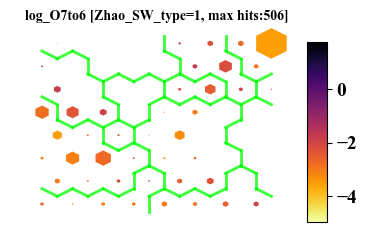
\includegraphics[width=4cm]{Roberts/SWtype-Zhao_SW_type-1-log_O7to6} &
		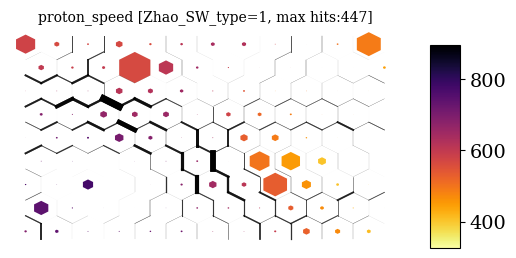
\includegraphics[width=4cm]{Roberts/SWtype-Zhao_SW_type-1-proton_speed}\hfill	\\
		ICME & & 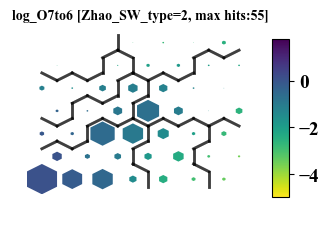
\includegraphics[width=4cm]{Roberts/SWtype-Zhao_SW_type-2-log_O7to6} &
		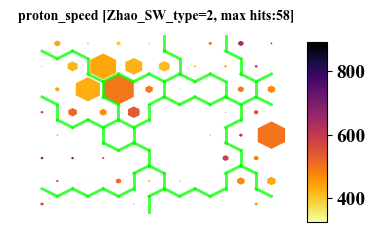
\includegraphics[width=4cm]{Roberts/SWtype-Zhao_SW_type-2-proton_speed}\hfill	\\
		NCHW & & 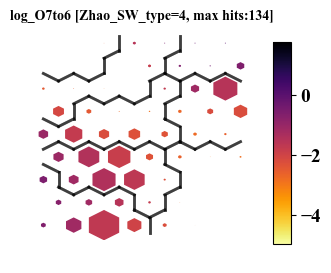
\includegraphics[width=4cm]{Roberts/SWtype-Zhao_SW_type-4-log_O7to6} &
		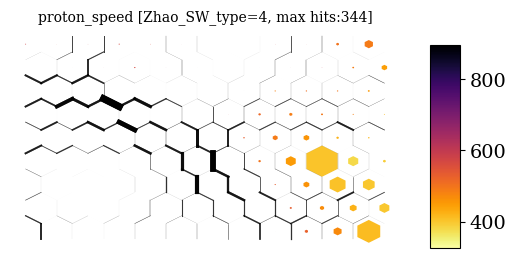
\includegraphics[width=4cm]{Roberts/SWtype-Zhao_SW_type-4-proton_speed}\hfill \\
		& $\log Sp$ & $\log V_{A}$ & $\log T_{\text{exp}}/T_p$ \\
		Streamer belt origin & 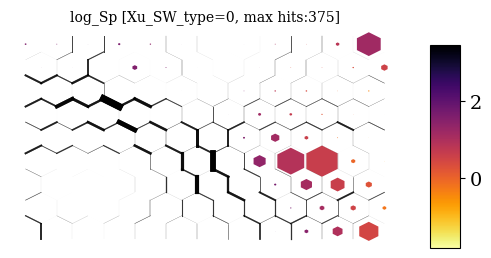
\includegraphics[width=4cm]{Roberts/SWtype-Xu_SW_type-0-log_Sp} &
		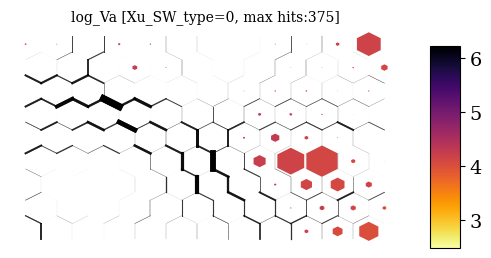
\includegraphics[width=4cm]{Roberts/SWtype-Xu_SW_type-0-log_Va} &
		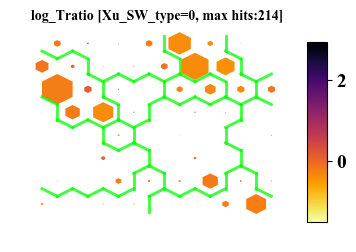
\includegraphics[width=4cm]{Roberts/SWtype-Xu_SW_type-0-log_Tratio} \hfill	\\
		
		Coronal hole origin & 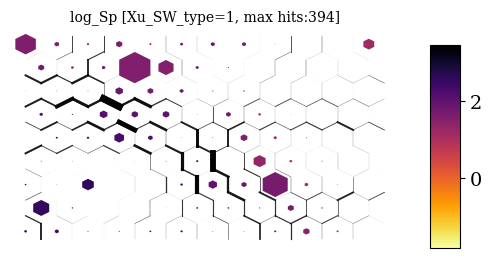
\includegraphics[width=4cm]{Roberts/SWtype-Xu_SW_type-1-log_Sp} &
		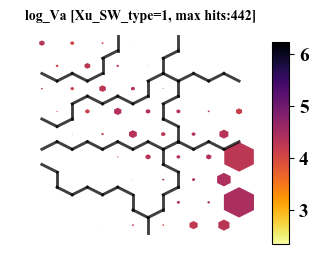
\includegraphics[width=4cm]{Roberts/SWtype-Xu_SW_type-1-log_Va} &
		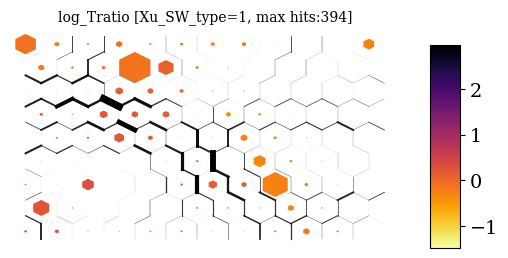
\includegraphics[width=4cm]{Roberts/SWtype-Xu_SW_type-1-log_Tratio} \hfill	\\
		
		Ejecta & 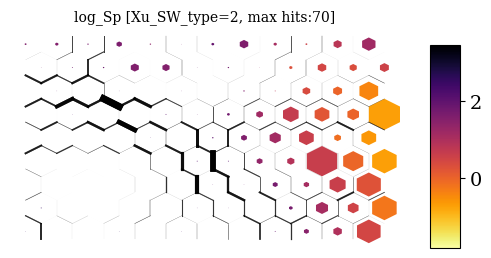
\includegraphics[width=4cm]{Roberts/SWtype-Xu_SW_type-2-log_Sp} &
		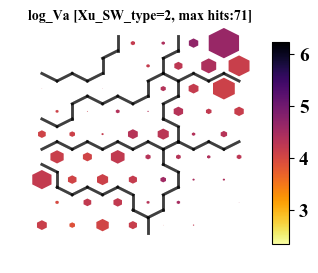
\includegraphics[width=4cm]{Roberts/SWtype-Xu_SW_type-2-log_Va} &
		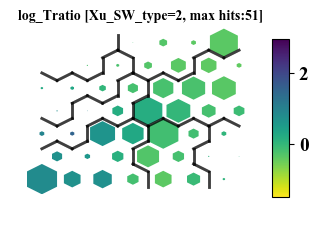
\includegraphics[width=4cm]{Roberts/SWtype-Xu_SW_type-2-log_Tratio} \hfill	\\
		
		Sector reversal origin & 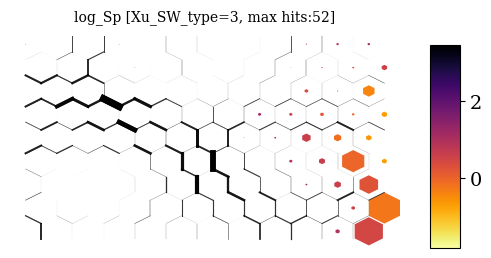
\includegraphics[width=4cm]{Roberts/SWtype-Xu_SW_type-3-log_Sp} &
		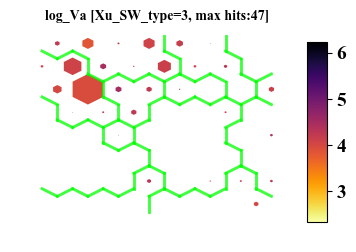
\includegraphics[width=4cm]{Roberts/SWtype-Xu_SW_type-3-log_Va} &
		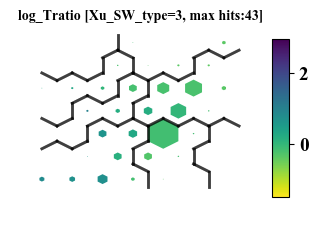
\includegraphics[width=4cm]{Roberts/SWtype-Xu_SW_type-3-log_Tratio} \hfill	\\
	\end{tabular}
\end{figure}
\end{document}%